\documentclass[12pt]{article}
\usepackage{kotex, inputenc, geometry, graphicx, cite}
% subfigure를 쓰기 위해서
\usepackage{subfigure}
% url 링크 걸기를 위해서 \url{링크} \href{링크 url}{링크를 걸 문장}
\usepackage{hyperref}

% 문서의 여백 설정
\geometry{
	a4paper,
	left = 19.1mm,
	right = 19.1mm,
	top = 25.4mm,
	bottom = 25.4mm
}
% 일관된 indent를 위해 indent를 모두 지움
\setlength{\parindent}{0cm}

% 문서 본문의 시작
\begin{document}
	
\section{과제 목적}
3종의 꽃의 4 feature로 구성된 주어진 data를 가지고 training하여,
feature를 통해 꽃의 종을 분류하는 NAIVE BAYESIAN CLASSIFIER를 디자인한다.
각 feature는 가우시안 분포를 따른다고 가정하며 bayesian theorem을 이용해서 확률을 계산한다. 

\section{코드 설명}

\subsection{feature\_normalization 함수}
\begin{figure}[h]
	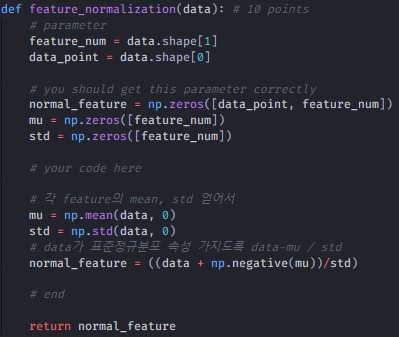
\includegraphics[width=0.7\textwidth]{figures/image01.png}
\end{figure}
입력받은 data를 각 feature에 대해 정규화해서 반환하는 함수이다.
각 feature data 값에 평균을 빼고 표준편차로 나누어서,
해당 feature에 대한 data가 평균이 0이고 표준편차가 1인 표준 정규분포를 따르도록 할 수 있다.

\subsection{split\_data 함수}
\begin{figure}[h]
	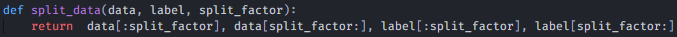
\includegraphics[width=\textwidth]{figures/image02.png}
\end{figure}
입력받은 data와 label을 split\_factor를 기준으로 분할해서 반환하는 함수이다.
training을 통해 classifier를 디자인한 다음에는 구현한 classifier가 얼마나 정확한지 test가 필요하므로,
미리 data를 어디에 사용할 것인지 구분해놓을 필요가 있다.

\subsection{get\_normal\_parameter 함수}
\begin{figure}[h]
	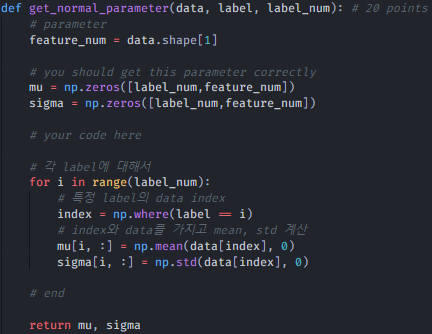
\includegraphics[width=10cm]{figures/image03.png}
\end{figure}
data와 label을 입력받아서 각 label에 해당하는 data의 평균과 분산을 반환하는 함수이다.
data를 classify하기 위해서는 각 label에 해당하는 data의 분포가 어떤 형태를 띄고 있는지 알아야 한다.
data의 분포를 통해 새로운 data가 어느 label에 해당할 확률이 높은지 계산할 수 있기 때문이다.

\subsection{get\_prior\_probability 함수}
\begin{figure}[h]
	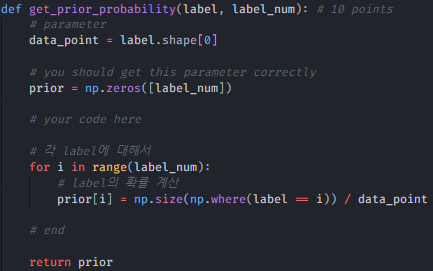
\includegraphics[width=10cm]{figures/image04.png}
\end{figure}
label을 입력받아서 prior를 계산해서 반환하는 함수이다.
prior는 각 label이 나올 확률이다.

\subsection{Gaussian\_PDF 함수}
\begin{figure}[h]
	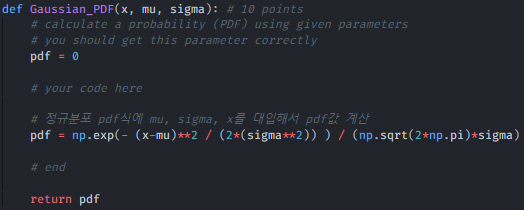
\includegraphics[width=0.7\textwidth]{figures/image05.png}
\end{figure}
x, mu, sigma를 입력받아 mu, sigma를 parameter로 하는 gaussian pdf에 x를 대입했을 때의 결과값을 반환하는 함수이다.

\subsection{Gaussian\_Log\_PDF 함수}
\begin{figure}[!h]
	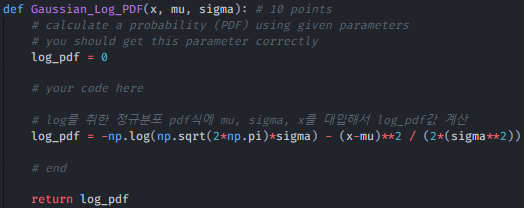
\includegraphics[width=0.7\textwidth]{figures/image06.png}
\end{figure}
x, mu, sigma를 입력받아 mu, sigma를 parameter로 하는 gaussian pdf에 x를 대입했을 때의 결과값을 log를 취해 반환하는 함수이다.

\subsection{Gaussian\_NB 함수}
\begin{figure}[!h]
	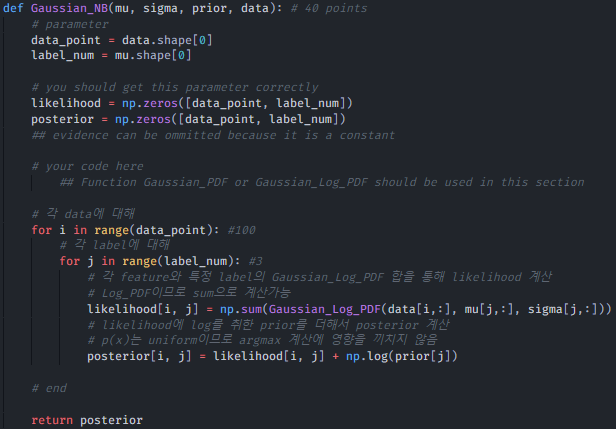
\includegraphics[width=0.8\textwidth]{figures/image07.png}
\end{figure}
입력받은 mu, sigma, prior, data를 가지고 posterior를 계산해서 반환하는 함수이다.
먼저 Gaussian\_PDF 함수 또는 Gaussian\_Log\_PDF 함수를 이용해서
특정 data의 feature값들의 각 label에 대한 유사도 likelihood를 계산한다.
그리고 likelihood 값에 prior을 추가해서 posterior를 계산한다.
BAYESIAN에서는 p(x)를 나누어주지만, p(x)가 모든 data에서 동일하여 classifier에 영향을 끼치지 않는다.
Gaussian\_PDF 함수를 사용하면 각 확률값을 곱하고,
Gaussian\_Log\_PDF 함수를 사용하면 각 확률값에 log를 취해서 더해준다.

\subsection{classifier 함수}
\begin{figure}[!h]
	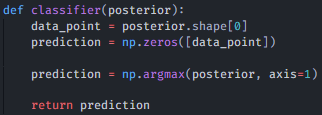
\includegraphics[width=10cm]{figures/image08.png}
\end{figure}
data별 posterior의 값을 비교해서 posterior가 최대가 되는 위치를 반환하는 함수이다.
data의 label별로 posterior값을 계산했으므로,
posterior가 가장 큰 위치의 label에 속한다고 판단할 수 있다. 

\subsection{accuracy 함수}
\begin{figure}[!h]
	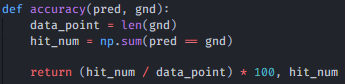
\includegraphics[width=10cm]{figures/image09.png}
\end{figure}
pred(예측값), gnd(실제값)을 비교해서 정확도를 측정하는 함수이다.

\section{실행 결과}
\begin{figure}[!h]
	\centering
    \subfigure{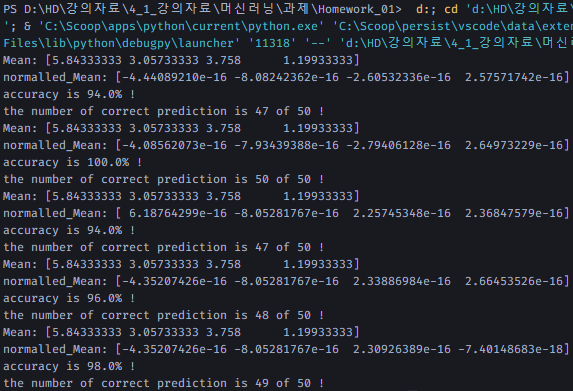
\includegraphics[width=0.6\textwidth]{figures/image10.png}}
    \subfigure{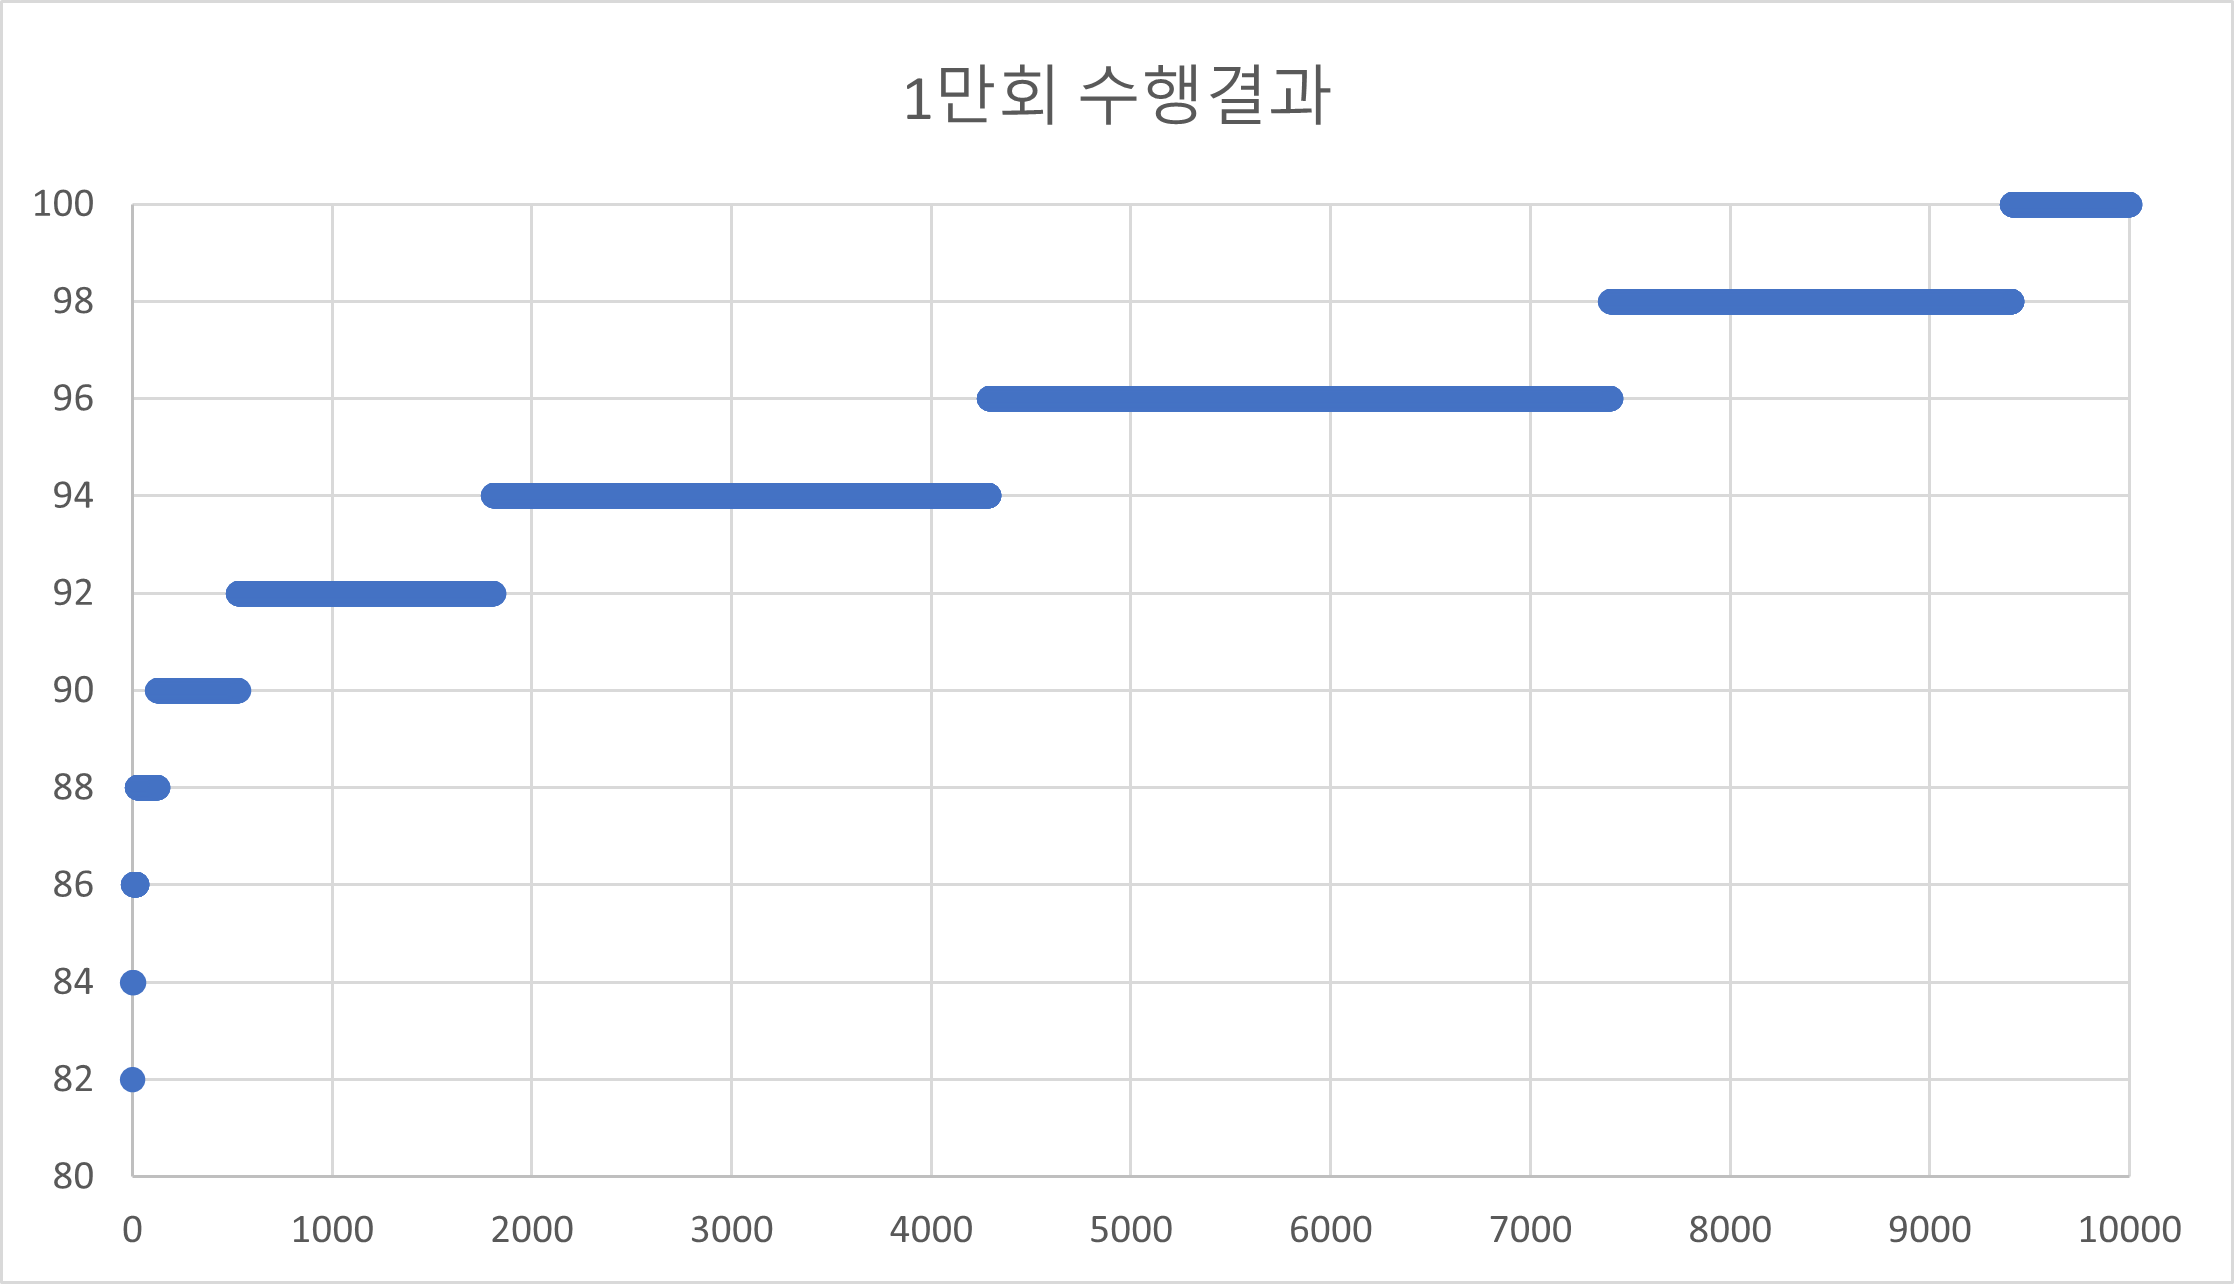
\includegraphics[width=0.6\textwidth]{figures/image11.png}}
    \caption{(a) 콘솔 출력 결과 (b) 1만회 수행 결과}
\end{figure}
1만번 training 및 test를 수행해본 결과 98.75\%가 90\% 이상의 정확도를 보였다.

% 인용 번호 없이 문서 인용
\nocite{wikipedia}

% Reference 출력
\bibliographystyle{unsrt}
\bibliography{ref}
	
\end{document}
